\documentclass[examplefnt,biber]{nowfnt} 

\usepackage[utf8]{inputenc}

\def\GD{\texttt{GD}}
\def\SGD{\texttt{SGD}}

%\usepackage[utf8]{inputenc} % allow utf-8 input
%\usepackage[T1]{fontenc}    % use 8-bit T1 fonts
\usepackage{amsthm}
\usepackage{amsmath}
\usepackage{amssymb}
\usepackage{amsfonts}
\usepackage{color}
\usepackage{fullpage}

\def\rc{\color{red}}
\def\bc{\color{blue}}

\usepackage{tikz,lipsum,lmodern}
\usepackage[most]{tcolorbox}

\def\bBoxBass{\begin{tcolorbox}[colback=blue!5!white,colframe=black!75!black] \begin{assumption}}
\def\bBoxEass{\end{assumption}\end{tcolorbox}}

\DeclareMathOperator*{\Argmax}{Argmax}
\DeclareMathOperator*{\Argmin}{Argmin}
\DeclareMathOperator*{\argmax}{argmax}
\DeclareMathOperator*{\argmin}{argmin}

\def\1{{\bf 1}}
\def\0{{\bf 0}}
\renewcommand{\a}{{\bf a}}
\renewcommand{\b}{{\bf b}}
\renewcommand{\c}{{\bf c}}
\renewcommand{\d}{{\rm d}}  % for derivatives
\newcommand{\e}{{\bf e}}
\newcommand{\f}{{\bf f}}
\newcommand{\g}{{\bf g}}
\newcommand{\h}{{\bf h}}
\newcommand{\bi}{{\bf i}}
\newcommand{\bj}{{\bf j}}
\newcommand{\bK}{{\bf K}}
%\newcommand{\k}{{\bf k}}
% in Latex2e this must be renewcommand
\renewcommand{\k}{{\bf k}}
\newcommand{\m}{{\bf m}}
\newcommand{\mhat}{{\overline{m}}}
\newcommand{\tm}{{\tilde{m}}}
\newcommand{\n}{{\bf n}}
\renewcommand{\o}{{\bf o}}
\newcommand{\p}{{\bf p}}
\newcommand{\q}{{\bf q}}
\renewcommand{\r}{{\bf r}}
\newcommand{\s}{{\bf s}}
\renewcommand{\t}{{\bf t}}
\renewcommand{\u}{{\bf u}}
\renewcommand{\v}{{\bf v}}
\newcommand{\w}{{\bf w}}
\newcommand{\x}{{\bf x}}
\def\X{{\bf X}}
\newcommand{\y}{{\bf y}}
\newcommand{\z}{{\bf z}}
\newcommand{\bl}{{\bf l}}
\newcommand{\A}{{\bf A}}
\newcommand{\B}{{\bf B}}
\newcommand{\C}{{\bf C}}
\newcommand{\D}{{\bf D}}
\newcommand{\Dcal}{\mathcal{D}}
%\newcommand{\E}{{\bf E}}
\newcommand{\F}{{\bf F}}
\newcommand{\G}{{\bf G}}
\newcommand{\Gcal}{{\mathcal{G}}}
\renewcommand{\H}{{\bf H}}
\newcommand{\I}{{\bf I}}
\newcommand{\J}{{\bf J}}
\newcommand{\K}{{\bf K}}
\renewcommand{\L}{{\bf L}}
%\newcommand{\Lcal}{{\mathcal{L}}}
\newcommand{\M}{{\bf M}}
\newcommand{\Mcal}{{\mathcal{M}}}
\newcommand{\N}{\mathcal{N}}  % for normal density
%\newcommand{\N}{{\bf N}}
\newcommand{\bupeta}{\boldsymbol{\upeta}}
\renewcommand{\O}{{\bf O}}
\renewcommand{\P}{{\bf P}}
\newcommand{\Q}{{\bf Q}}
\newcommand{\R}{{\bf R}}
\renewcommand{\S}{{\bf S}}
\newcommand{\Scal}{{\mathcal{S}}}
\newcommand{\T}{{\bf T}}
\newcommand{\Tcal}{{\mathcal{T}}}
\newcommand{\U}{{\bf U}}
\newcommand{\Ucal}{{\mathcal{U}}}
\newcommand{\tU}{{\tilde{\U}}}
\newcommand{\tUcal}{{\tilde{\Ucal}}}
\newcommand{\V}{{\bf V}}
\newcommand{\W}{{\bf W}}

\def\dd{\rm D}

\def\E{\mathbb{E}}

\def\({\left(}
\def\){\right)}
\def\1{{\bf 1}}

\def\Ocal{\mathcal{O}}

%% theorem format %%
\newcounter{ass_counter}
\newcounter{thm_counter}
\newcounter{remark_counter}
%\newtheorem{theorem}[thm_counter]{Theorem}%[section]
% \newtheorem{lemma}[thm_counter]{Lemma}%[Lemma]
% \newtheorem{corollary}[thm_counter]{Corollary}
\newtheorem{assumption}[ass_counter]{Assumption}
% \newtheorem{remark}[remark_counter]{Remark}
% \newtheorem{proposition}[thm_counter]{Proposition}

%% display %%
\allowdisplaybreaks
\newcommand\numberthis{\addtocounter{equation}{1}\tag{\theequation}}



\title{Distributed Learning with
First-order Methods: An Overly Simplified  Introduction}

\subtitle{Systems and Theory}

\maintitleauthorlist{
Ji Liu \\
XXX \\
email \\
\and
Ce Zhang \\
ETH Zurich \\
ce.zhang@inf.ethz.ch
}

\issuesetup
{%
 copyrightowner={A.~Heezemans and M.~Casey},
 volume        = xx,
 issue         = xx,
 pubyear       = 2018,
 isbn          = xxx-x-xxxxx-xxx-x,
 eisbn         = xxx-x-xxxxx-xxx-x,
 doi           = 10.1561/XXXXXXXXX,
 firstpage     = 1, %Explain
 lastpage      = 18
 }

\addbibresource{sample-now.bib}

\usepackage{mwe}

%AUTHORS FOR ABSTRACT PAGE
\author[1]{Liu,Ji}
\author[2]{Zhang,Ce}

\affil[1]{XXX;email}
\affil[2]{ETH Zurich; ce.zhang@inf.ethz.ch}

\articledatabox{\nowfntstandardcitation}

\begin{document}

\makeabstracttitle

\begin{abstract}
Scalable and efficient distributed learning
is one of the main driving forces behind
the recent rapid advancement of machine learning and artificial intelligence. One prominent feature of this
topic is that recent progresses have been
made by researchers in {\em two} communities:
(1) {\em the system community} such as database,
data management, and distributed systems, and
(2) {\em the machine learning and
mathematical optimization community}. 
The interaction and knowledge sharing
between these two communities lead to the
rapid development of new distributed learning
systems and theory.

In this paper, we hope to provide a 
brief introduction of some distributed
learning techniques that have recently
been developed. One special focus on this
work is to make sure that this paper can
be easily understood by researchers
in {\em both} communities --- On the system
side, we rely on a simplified system model,
which hides many system details that might
not be necessary for the reader to understand
the intuition behind the system speedups;
On the theory side, we rely on minimal 
assumptions and significantly 
simplified the proof of some recent work
to achieve comparable result. 
\end{abstract}

\chapter{Introduction}

\section{Machine Learning and
Optimization}

\section{Gradient Descent 
and Stochastic Gradient Descent}
Objective
\begin{align}
\min_{\x \in \mathbb{R}^d}\quad \left\{f(\x):=\sum_{m=1}^M F_m(\x)\right\}
\label{eq:obj-gd}
\end{align}

Let $f^\star := {1\over M}\min_{\x} f(\x)$.

The gradient descent ($\GD$) can be described below
\begin{align}
(\GD)\quad\x_{t+1} = \x_t - \gamma f'(\x_t)
\label{eq:gd}
\end{align}
where $t$ is the iteration index.
{\rc TODO two intuitions about the gradient descent algorithms.}

To compute the gradient of $f'(\x):={1\over M} F'_m(\x)$, the typical computational complexity is $O(Md)$ where $M$ is the number of samples and $d$ the dimension of the model $\x$. 
The typical computational complexity to compute the gradient is $O(Md)$. To see the reason, let us imagine the naive linear regression with $F_m:= {1\over 2}(\a_m^\top \x -b)^2$ and the gradient $f'(\x):={1\over M}\sum\a_m(\a_m^\top \x - b)$.

\begin{tcolorbox}[colback=pink!5!white,colframe=black!75!black]
\begin{assumption} \label{ass:gd}
We make assumptions in the following:
\begin{itemize}
\item ({\bf Lipschitz gradient}) The objective function is assume to have Lipschitz gradient, that is, there exists a constant $L$ satisfying
\begin{align*}
f(\y) - f(\x) \leq \langle f'(\x), \y-\x \rangle + {L\over 2} \|\y - \x\|^2 \quad \forall \x, \forall\y
\end{align*}
\item ({\bf Smoothness}) All functions $F_m(\cdot)$'s are smooth.
\end{itemize}
%\item ({\bf Bounded $f(\x)$ from below})
\end{assumption}
\end{tcolorbox}
The smoothness assumption on $F_m(\cdot)$'s implies that the overall objective function $f(\cdot)$ is smooth too.

{\rc TODO Intuition of assumptions}

We apply the Lipschitz gradient assumption and obtain the following golden inequality immediately
\begin{align*}
f(\x_{t+1}) - f(\x_{t}) \leq & \langle f'(\x_{t}), \x_{t+1} - \x_t  \rangle + {L\over 2}\|\x_{t+1} - \x_t\|^2
\\ = &
- \gamma \| f'(\x_t) \|^2 + {\gamma^2 L \over 2} \|f'(\x_t)\|^2
\\ = &
-\gamma\left(1- {\gamma L\over 2}\right) \|f'(\x_t)\|^2
\numberthis
\label{eq:gd_proof_1}
\end{align*}
We can see that as long as the learning rate $\gamma$ is small enough such that $1-{\gamma L}/2 > 0$, $f(\x_{t+1})$ can improve $f(\x_t)$. Therefore, the learning cannot be too large to guarantee the progress in each step. However, it is also a bad idea if the learning rate is over small, since the progress is proportional to $\gamma (1-\gamma L /2)$. The optimal learning rate can be obtained by simply maximizing 
\[
\gamma (1-\gamma L /2)
\]
over $\gamma$, which gives the optimal learning rate for gradient descent method $\gamma^{\star} = 1/L$. Substituting $\gamma = \gamma^\star$ into \eqref{eq:gd_proof_1} yields
\begin{align*}
f(\x_{t+1}) - f(\x_t) \leq -{1 \over 2L} \|f'(\x_t)\|^2
\end{align*}
or equivalently 
\begin{align}
f(\x_{t}) - f(\x_{t+1}) \geq {1 \over 2L} \|f'(\x_t)\|^2.
\label{eq:gd_proof_2}
\end{align}
% Acute readers may ask how do I know the value of the Lipschitz constant $L$. Unfortunately, it is usually unknown. However, in most practical scenarios, it is not hard to find an upper for $L$.

Summarizing Eq.~\eqref{eq:gd_proof_2} over $t$ from $t=1$ to $t=T$ yields
\begin{align*}
{1\over 2L} \sum_{t=1}^T \|f'(\x_t)\|^2 \leq & \sum_{t=1}^T\left(f(\x_{t}) - f(\x_{t+1})\right)  
\\ = &
f(\x_1) - f(\x_{t+1})
\\ \leq &
f(\x_1) - f^\star.
\end{align*}
Rearranging the inequality yields the following convergence rate for gradient descent
\begin{tcolorbox}[colback=blue!5!white,colframe=black!75!black]
\begin{theorem}
Under Assumption~\ref{ass:gd}, the gradient descent method admits the following convergence rate
\begin{align}
{1\over T}\sum_{t=1}^T\|f'(\x_t)\|^2 \lesssim {L \over T}(f(\x_1) - f^{\star})
\end{align}
by choosing the learning rate $\gamma = {1\over L}$.
\end{theorem}
\end{tcolorbox}
This result indicates that the averaged gradient norm converges in the rate of $1/T$.

There are two major disadvantages for the $\GD$ method:
\begin{itemize}
\item The computational complexity and system overhead are too high in each iteration to compute a single gradient;
\item For nonconvex objectives, the gradient descent often stick on bad (shallow) local optimum.
\end{itemize}

To overcome these issues, the stochastic gradient method $\SGD$ is widely used in machine learning training. Instead of computing a full gradient in each iteration, people only compute the gradient on a (or a few number of) sampled data. In particular, people randomly sample an $m\in [M]$ independently each time and update the model by
\begin{align}
(\SGD)\quad \x_{t+1} = \x_t - \gamma F'_{m_t}(\x_t)
\label{eq:sgd}
\end{align}
where $m_t$ denotes the index randomly selected at the $t$th iteration. $F'_{m_t}(\x_t)$ is called stochastic gradient. We use $g(\x)$ (or $g_t(\x)$) denote the stochastic gradient (or at the $t$th iteration) for short. An important property for stochastic gradient is that its expectation is equal to the true gradient, that is,
\begin{align}
\E[g(\x)] = \E_{m} [F'_{m}(\x)] = f'(\x) \quad \forall \x.
\end{align}
%<<<<<<< HEAD
An immediate advantage of $\SGD$ is that the computational complexity reduces to $O(d)$ per iteration. It is worth pointing out that the $\SGD$ algorithm is NOT a descent algorithm due to the randomness.

The next question is whether it converges and how fast if yes. We first make some typical assumption
\begin{tcolorbox}[colback=pink!5!white,colframe=black!75!black]
\begin{assumption} \label{ass:sgd}
%=======
%An clear advantage of $\SGD$ is that the computational complexity reduces to $O(d)$ per iteration. It is worth pointing out that the $\SGD$ algorithm is NOT a descent algorithm due to the randomness.
%
%The next question is whether it converges and how fast if yes. We first make some typical assumption
%\begin{tcolorbox}[colback=pink!5!white,colframe=black!75!black]
%\begin{assumption}
%>>>>>>> b94b8679f310fa566039184f25fe4da4b1ce56ff
We make the following assumption:
\begin{itemize}
\item ({\bf Bounded stochastic variance}) The stochastic gradient is with bounded variance, that is, there exists a constant $\sigma$ satisfying
\[
\E[\|g(\x) - f'(\x)\|^2] \leq \sigma^2\quad \forall \x
\]
\end{itemize}
\end{assumption}
\end{tcolorbox}

\begin{align*}
f(\x_{t+1}) - f(\x_{t}) \leq & \langle f'(\x_{t}), \x_{t+1} - \x_t  \rangle + {L\over 2}\|\x_{t+1} - \x_t\|^2
\\ = &
-\gamma \langle f'(\x_t), g_t(\x_t) \rangle + {L\gamma^2\over 2} \|g_t(\x_t)\|^2. \numberthis 
\label{eq:sgd_proof_1}
\end{align*}
Note two important properties
\begin{itemize}
\item $\E[\langle f'(\x_t), g_t(\x_t) \rangle] = \langle f'(\x_t), \E[g_t(\x_t)] \rangle =  \|f'(\x_t)\|^2$
\item $\E[\|g_t(\x_t)\|^2] = \|f'(\x_t)\|^2 + \E[\|g_{t}(\x_t) - f'(\x_t)\|^2] \leq \|f'(\x_t)\|^2 + \sigma^2$,
\end{itemize}
where the second property uses the property of variance, that is, any random variable vector $\xi$ satisfies 
\begin{align}
\E[\|\xi\|^2] = \|\E[\xi]\|^2 + \E[\|\xi- \E[\xi]\|]^2.
\label{eq:mean-var}
\end{align}
Apply these two properties to \eqref{eq:sgd_proof_1} and take expectation on both sides:
\begin{align*}
& \E[f(\x_{t+1})] - \E[f(\x_t)] 
\\ \leq & 
-\gamma \E[\|f'(\x_t)\|^2] + {L\gamma^2 \over 2} \left(\E[\|f'(\x_t)\|^2] + \sigma^2 \right) \numberthis \label{eq:sgd_proof_2}
\\ \leq &
-\gamma\left(1 - {\gamma L \over 2}\right)  \E[\|f'(\x_t)\|^2] + {\gamma^2 \over 2} L\sigma^2. \numberthis \label{eq:sgd_proof_2}
\end{align*}
From \eqref{eq:sgd_proof_2}, we can see that $\SGD$ does not guarantee ``descent'' in each iteration unlike $\GD$, but it guarantees ``descent'' in the expectation sense in each iteration as long as $\gamma$ is small enough and $\|f'(\x_t)\|^2 > 0$. This is because the first term in \eqref{eq:sgd_proof_2} is in the order of $O(\gamma)$ while the second term is in the order of $O(\gamma^2)$.

Next we summarize \eqref{eq:sgd_proof_2} from $t=1$ to $t=T$ and obtain
\begin{align}
\E[f(\x_{T+1})] - f(\x_1) \leq -\gamma\left(1-{\gamma L \over 2} \right)\sum_{t=1}^T\E[\|f'(\x_t)\|^2] + {\gamma^2 \over 2} TL\sigma^2.
\label{eq:sgd_proof_3}
\end{align}
We choose the learning rate $\gamma = {1\over L+ \sigma\sqrt{TL}}$ while implies that $(1-\gamma L/2)> 1/2$. It follows
%to simply the right hand side of \eqref{eq:sgd_proof_3}
\begin{align*}
&{1\over T} \sum_{t=1}^T\E[\|f'(\x_t)\|^2] 
\\ \lesssim & 
\frac{f(\x_1)- \E[f(\x_{T+1})]}{T\gamma} + \gamma L\sigma^2
\\  \lesssim &
\frac{f(\x_1)- f^\star}{T\gamma} + \gamma L\sigma^2
\\ \lesssim &
{(f(\x_1) - f^\star)L \over T} + {(f(\x_1) - f^\star)\sqrt{L}\sigma \over \sqrt{T}}. 
\end{align*}
Therefore the convergence rate of $\SGD$ can be summarized into the following theorem
\begin{tcolorbox}[colback=blue!5!white,colframe=black!75!black]
\begin{theorem}
Under Assumptions~\ref{ass:gd} and \ref{ass:sgd}, the $\SGD$ method admits the following convergence rate
\begin{align}
{1\over T}\sum_{t=1}^T\E[\|f'(\x_t)\|^2] \lesssim {(f(\x_1) - f^\star)L \over T} + {(f(\x_1) - f^\star)\sqrt{L}\sigma \over \sqrt{T}}. 
\end{align}
by choosing the learning rate $\gamma = {1\over L+\sigma \sqrt{TL}}$.
\end{theorem}
\end{tcolorbox}
{\rc need to fix the learning rate.}
%=======
%-\gamma\left(1 - {\gamma L \over 2}\right)  \E[\|f'(\x_t)\|^2] + {L\gamma^2 \over 2} \sigma^2. \numberthis \label{eq:sgd_proof_2}
%\end{align*}
%From \eqref{eq:sgd_proof_2}, we can see that $\SGD$ does not guarantee ``descent'' in each iteration unlike $\GD$, but it guarantees ``descent'' in the expectation sense in each iteration as long as $\gamma$ is small enough and $\|f'(\x_t)\|^2 > 0$.
%
%
%
%>>>>>>> b94b8679f310fa566039184f25fe4da4b1ce56ff


 


\section{An Overly Simplified Distributed Communication Model}

\label{sec:commmodel}


In this article, we cover a diverse range of 
{\em system relaxations} techniques for 
distributed stochastic gradient descent systems.
From a mathematical optimization perspective, all
system relaxations we introduce {\em does not
make the convergence (loss vs. \# iterations / epochs) faster}.
\footnote{The reason
that we emphasize the ``mathematical optimization''
perspective is because that some researchers
find certain system relaxations can actually lead
to better generalization performance~\cite{XXX,XXX}.
We do not consider generalization in this article.}
%
Then {\em why do we even want to introduce these 
relaxations into our system in the first place?}

One common theme of the techniques we cover in
this article is that their goal is not
to improve the convergence rate in terms
of \# iterations / epochs, but instead, their
goal is to make each iteration finishes faster
in terms of wall clock time.
As a result, to reason about each system relaxation
techniques in this article, we need to first
agree on a {\em performance model} of the
underlying distributed system. In this Section,
we introduce a very simple performance model --- 
it ignores many (if not most) important system
characteristics, but is just informative enough
for readers to understand why each system relaxations
in this article actually makes a system faster.

\subsection{Assumptions}

\begin{figure}[t!]
\centering
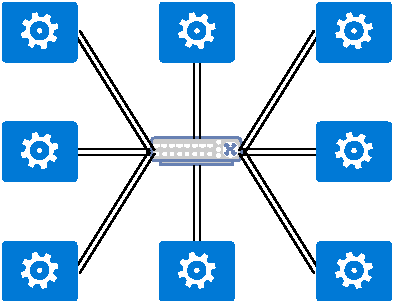
\includegraphics[width=0.3\textwidth]{figures/Chpt1.3/CommunicationModel.pdf}
\caption{An illustration of the distributed communication
model we use in this article. We assume that all devices
(worker, machine) are connected via a ``logical switch'',
whose property is defined in Section~\ref{sec:commmodel}}.
\label{fig:commmodel}
\end{figure}

Figure~\ref{fig:commmodel} illustrates our communication model. Each worker (blue rectangle)
corresponds to {\em one} computation device,
and all workers are connected via a ``logical switch''
that has the following property:
\begin{enumerate}
\item The switch has infinitely large bandwidth.
\item For each message that ``passes through''
the switch (send by worker $w_i$ and received
by worker $w_j$), the switch adds a constant
delay $t_{latency}$ independently of the number
of concurrent messages that this switch is 
serving. This delay is the difference
between the sender sending out the first bit
and the receiver receiving the first bit.
\end{enumerate}

For each worker, we also assume the following properties:
\begin{enumerate}
\item Each worker can only send one message 
at the same time.
\item Each worker can only receive messages 
at the same time.
\item Each worker can concurrently receive one 
message and send one message at the same time.
\item Each worker has a fixed bandwidth, i.e.,
to send / receive one unit (e.g., MB) amount of data,
it requires $t_{transfer\_1MB}$ seconds.
\end{enumerate}

\begin{figure}[t!]
\centering
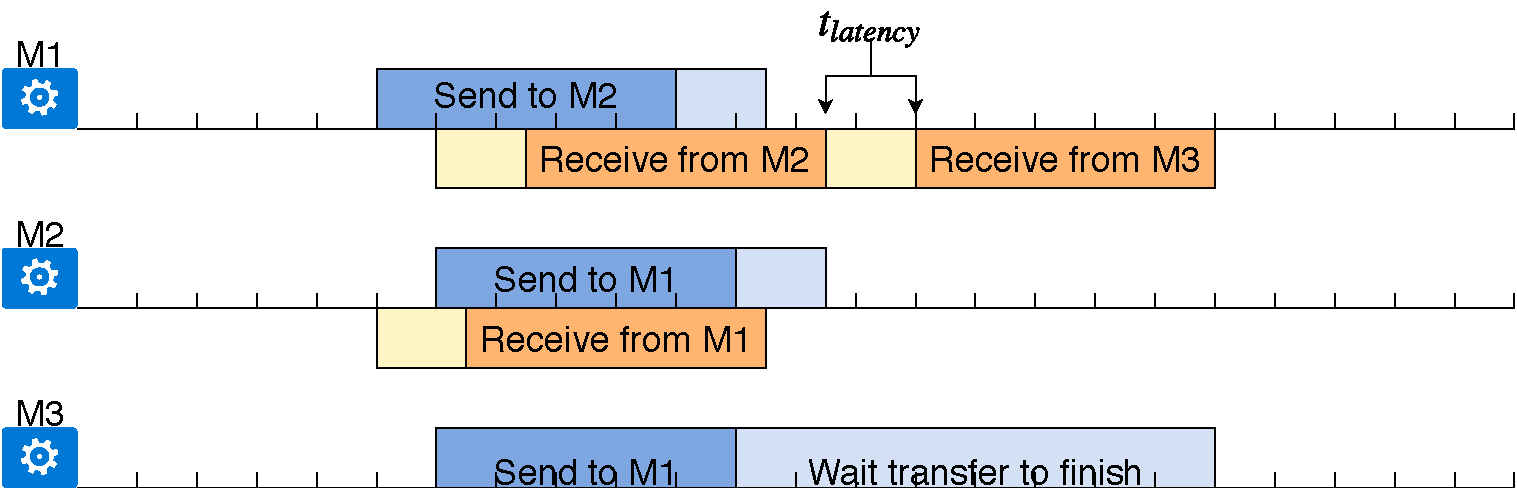
\includegraphics[width=1.0\textwidth]{figures/Chpt1.3/Communication_Illustration.pdf}
\caption{Illustration of the communication pattern of Example~\ref{exp:communication_illustration}.}
\label{fig:communication_illustration}
\end{figure}

\begin{figure}[t!]
\centering
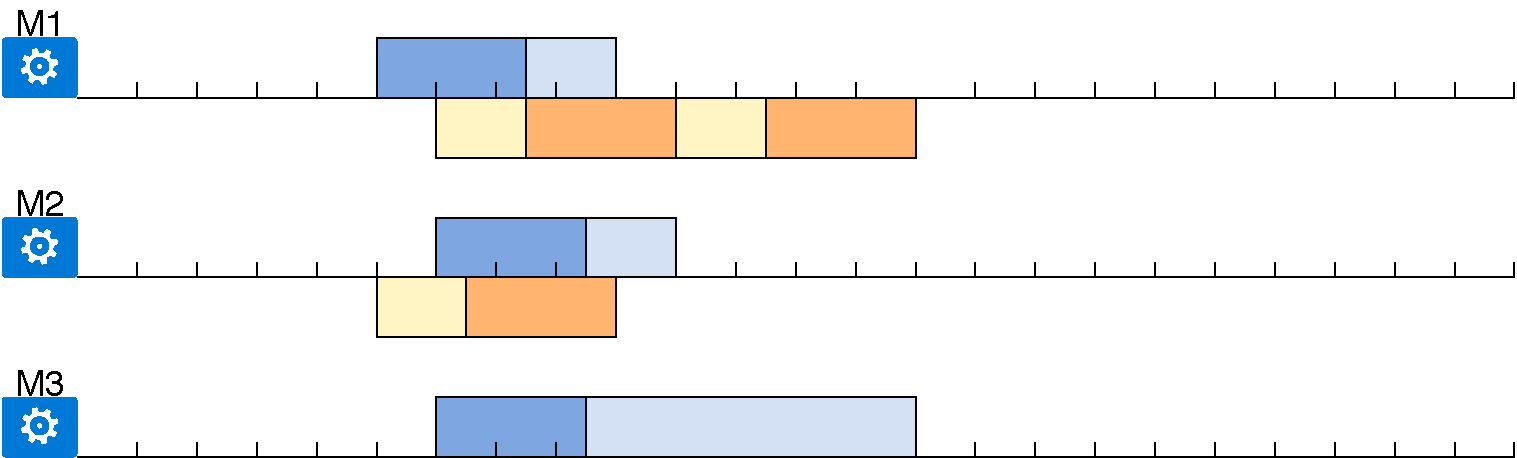
\includegraphics[width=1.0\textwidth]{figures/Chpt1.3/Communication_Illustration_lowPrecision.pdf}
\caption{Illustration of the communication pattern of Example~\ref{exp:communication_illustration}, with 2x data compression.}
\label{fig:communication_illustration_lowprecision}
\end{figure}

\begin{example} \label{exp:communication_illustration}
Under the above communication model,
Consider the following three events:
\begin{verbatim}
            time      event
            0:05      M1 send 1MB to M2
            0:06      M2 send 1MB to M1
            0:06      M3 send 1MB to M2
\end{verbatim}
We assume that the latency added by the switch $t_{latency}$
is 1.5 unit of time and it took 5 units of time to
transfer 1MB of data. 
Figure~\ref{fig:communication_illustration} illustrates 
the timeline on three machines under our communication 
model. The yellow block corresponds to the {\em latency}
added by the ``logical switch''. We also see that 
the machine \texttt{M1} can concurrently send (blue
block) and
receive data (orange block) at the same time; however,
when the machine \texttt{M3} tries to send data to
\texttt{M1}, because the machine \texttt{M2} is
sending data to \texttt{M1} already, \texttt{M3}
needs to wait (the shallow blue block of \texttt{M3}).
\end{example}

\begin{example} \label{exp:communication_illustration}
Figure~\ref{fig:communication_illustration_lowprecision}
illustrates a hypothetical scenario in which 
all data sent in Example~\ref{exp:communication_illustration}
are ``magically'' compressed by 2$\times$ at the sender.
As we will see in later chapters, this is similar to what 
would happen if one compresses the gradient by 2$\times$
during training.

We make multiple observations from Figure~\ref{fig:communication_illustration_lowprecision}.
\begin{enumerate}
\item First, compressing data does make the ``system'' faster.
Without compression, all three events finish in 14 units
of time (Figure~\ref{fig:communication_illustration})
whereas it finishes in 9 units of time after compress.
This is because the time used to {\em transfer}
the data is decreased by half, in our communication model.
\item Second, even if the data are compressed by 2$\times$,
the speedup of the system is smaller than that, in fact, it
is only $14/9 = 1.55\times$. This is because that, even 
though the transfer time is cut by half, the communication
latency does not decrease as a result of data compression.
\end{enumerate}
\end{example}

We now use the above communication model to describe
three popular ways of implementing distributed stochastic 
gradient descent. These implementations will often serve
as the baseline on which we apply different system relaxations
to remove certain system bottlenecks that raise in 
different configurations of $(t_{latency}, t_{transfer})$
together with the relative computational cost on each machine.

\begin{figure}[t!]
\centering
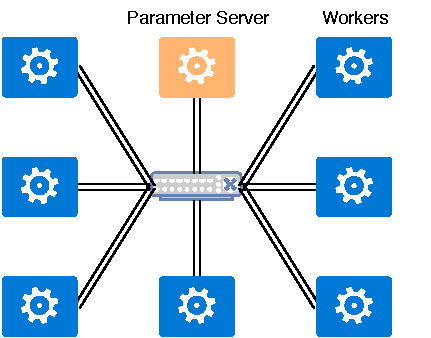
\includegraphics[width=0.3\textwidth]{figures/Chpt1.3/Communication_PS1.pdf}
\caption{Illustration of the parameter server architecture 
with a single dedicated parameter server.}
\label{fig:communication_illustration_ps1}
\end{figure}


\begin{figure}[t!]
\centering
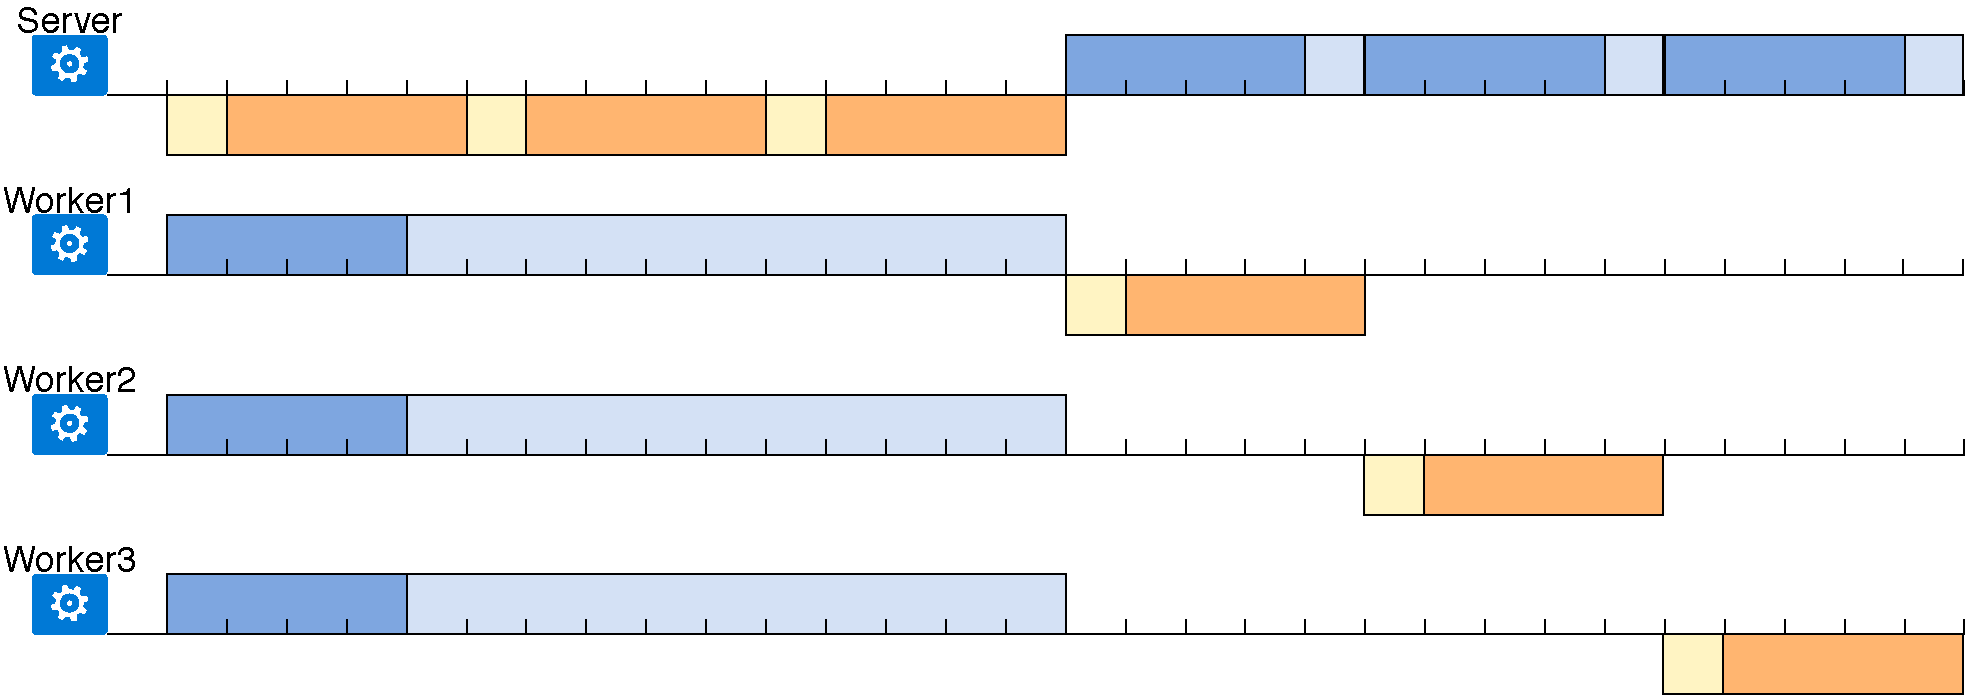
\includegraphics[width=1.0\textwidth]{figures/Chpt1.3/Communication_PS.pdf}
\caption{Illustration of the communication
pattern of the parameter server architecture 
with a single dedicated parameter server.}
\label{fig:communication_illustration_timeline_ps1}
\end{figure}


\begin{figure}[t!]
\centering
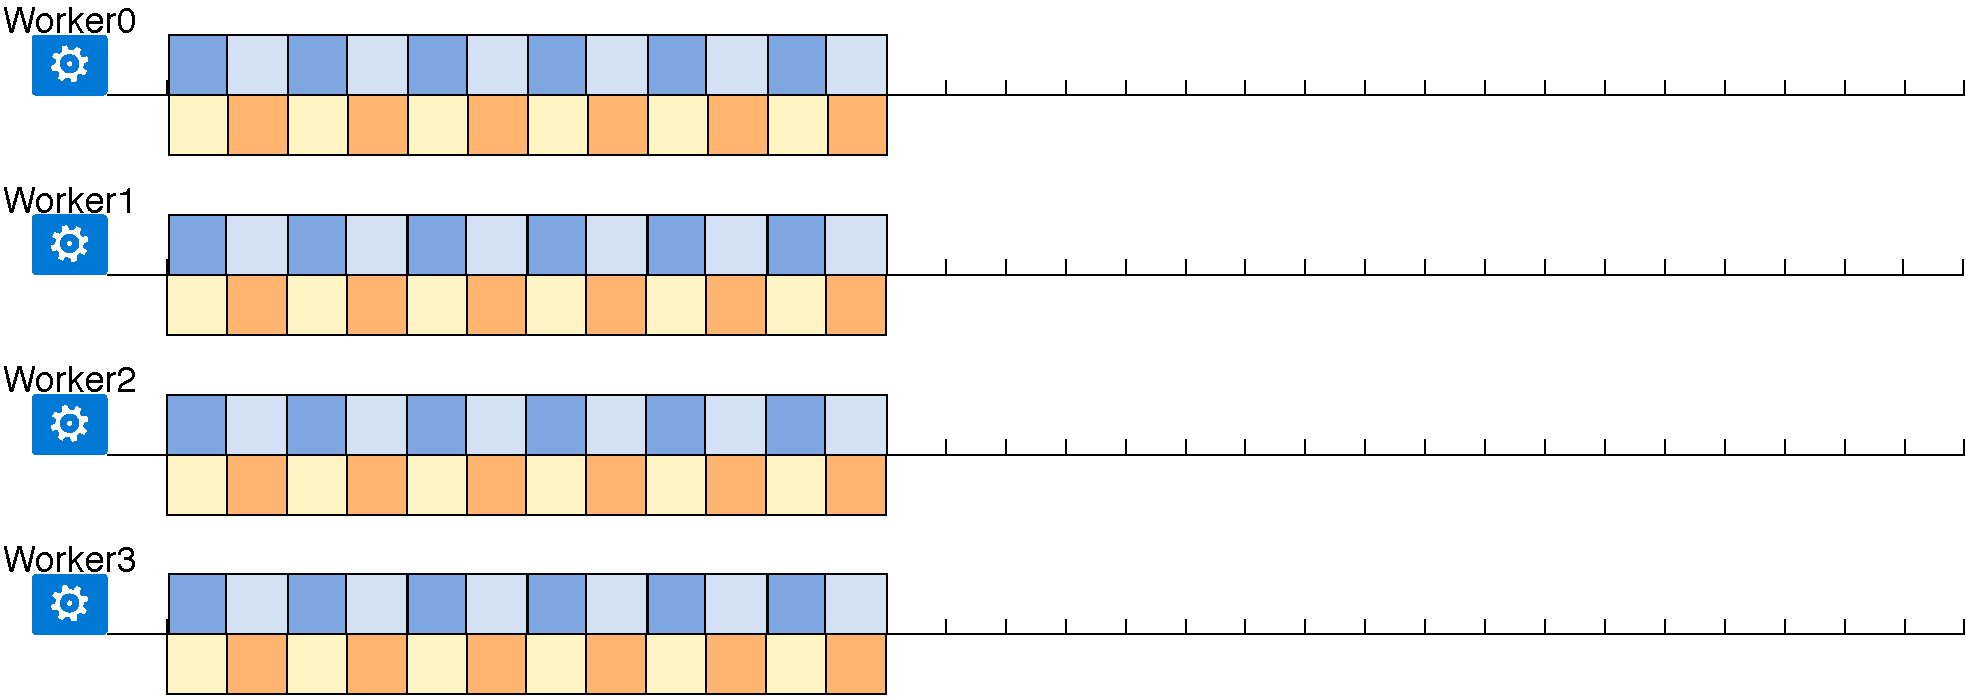
\includegraphics[width=1.0\textwidth]{figures/Chpt1.3/Communication_pattern_AllReduce.pdf}
\caption{Illustration of the communication
pattern of the AllReduce architecture with ring topology.}
\label{fig:communication_illustration_timeline_allreduce}
\end{figure}


\begin{figure}[t!]
\centering
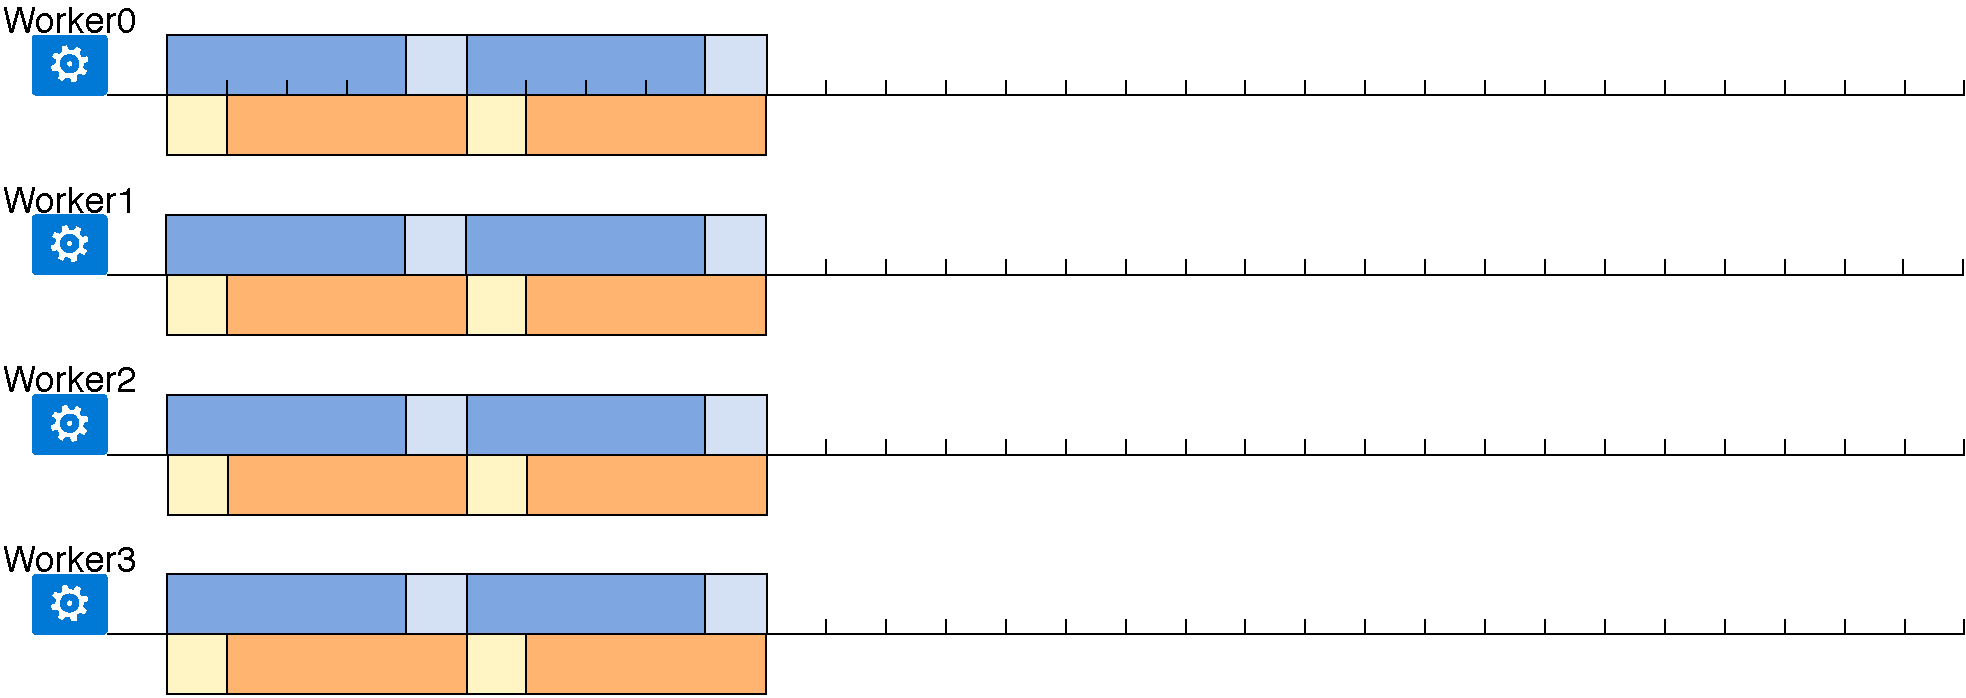
\includegraphics[width=1.0\textwidth]{figures/Chpt1.3/Communication_pattern_decentralized.pdf}
\caption{Illustration of the communication
pattern of the decentralized  architecture with ring topology.}
\label{fig:communication_illustration_timeline_decent}
\end{figure}
\subsection{Parameter Server}

\subsection{AllReduce}

\paragraph{Why Do We Partition the Model?}


\subsection{Multi-machine Parameter Server}










\chapter{Single Thread System}

\section{General Theoretical Framework}

\section{Stochastic Gradient
Descent}

\section{Low Precision Computation}

\section{Low Precision Data}

\section{System Implications}

\chapter{Distributed/Parallel System}

\section{General Theoretical Framework}

\section{Low Precision 
Communications}

\section{Asynchronous Communications}
\begin{align*}
\x_{t+1} = \x_t - \gamma g_t(\x_{\dd(t)})
\end{align*}

Important property for $g_t(\x_{\dd(t)})$
\begin{align}
\E[g_t(\x_{\dd(t)})] = f'(\x_{\dd(t)})
\end{align}

\begin{tcolorbox}[colback=pink!5!white,colframe=black!75!black]
\begin{assumption} \label{ass:asgd}
%=======
%An clear advantage of $\SGD$ is that the computational complexity reduces to $O(d)$ per iteration. It is worth pointing out that the $\SGD$ algorithm is NOT a descent algorithm due to the randomness.
%
%The next question is whether it converges and how fast if yes. We first make some typical assumption
%\begin{tcolorbox}[colback=pink!5!white,colframe=black!75!black]
%\begin{assumption}
%>>>>>>> b94b8679f310fa566039184f25fe4da4b1ce56ff
We make the following assumption:
\begin{itemize}
\item ({\bf Bounded staleness}) Assume that the staleness is bounded, that is,  
\[
0 \leq t - \dd(t) \leq \tau\quad \forall t
\]
where $\tau$ is a global parameter.
\end{itemize}
\end{assumption}
\end{tcolorbox}

\begin{align*}
f(\x_{t+1})- f(\x_t) \leq -\gamma \langle f'(\x_t),  g_t(\x_{\dd(t)})\rangle + {L\gamma^2 \over 2} \|g_t(\x_{\dd(t)})\|^2 
\end{align*}

Take expectation on both sides
\begin{align*}
\E[f(\x_{t+1})]- \E[f(\x_t)] \leq & -\gamma \E[\langle f'(\x_t),  g_t(\x_{\dd(t)})\rangle\ + {L\gamma^2 \over 2} \E[\|g_t(\x_{\dd(t)})\|^2] 
\numberthis \label{eq:asgd_proof_0}
%\\ = &
%\gamma \E[\langle f'(\x_t),  g(\x_{\dd(t)})\rangle] + {L\gamma^2 \over 2} \E[\|g_t{\x_{\dd(t)}}\|^2] 
% \\ = &
% \gamma \E[\langle f'(\x_t), f'(\x_{t_{\tau_t}})]
\end{align*}
We consider the items on the right hand side respectively. For $\E[\|g_t(\x_{\dd(t)})\|^2]$, we have
\begin{align*}
\E_{\dd(t)}[\|g_t(\x_{\dd(t)})\|^2] =&  \E_{\dd(t)}[\|\g_t(\x_{\dd(t)})-f'(\x_{\dd(t)})\|^2] + \|\f_t(\x_{\dd(t)})\|^2
\\ \leq &
\sigma^2 + \|\f_t(\x_{\dd(t)})\|^2,
\numberthis \label{eq:asgd_proof_1}
\end{align*}
where the first equality is due to the fact \eqref{eq:mean-var}, and the second one is due to the bounded variance assumption, that is, Assumption~\ref{ass:sgd}.

For $\E[\langle f'(\x_t),  g(\x_{\dd(t)})\rangle]$, we have
\begin{align*}
& \E[\langle f'(\x_t),  g(\x_{\dd(t)})\rangle] 
\\= & 
\E[\langle f'(\x_t),  \E_{\dd(t)}[g(\x_{\dd(t)})]\rangle]
\\= & 
\E[\langle f'(\x_t), f'(\x_{\dd(t)})\rangle]
\\ = &
 \E\left[{1\over 2}\|f'(\x_t) - f'(\x_{\dd(t)})\|^2 - {1\over 2}\|f'(\x_t)\|^2 - {1\over 2}\|f'(\x_{\dd(t)})\|^2 \right]
 \numberthis \label{eq:asgd_proof_2}
%\E[\langle f'(\x_t),  f'(\x_t)\rangle] + \E[\langle f'(\x_t), f'(\x_{\dd(t)}) - f'(\x_t)\rangle]
%\\ = &
%\E [\|f'(\x_t)\|^2] + \E [\|f'(\x_t)]
\end{align*}
The last equality uses an important property
\begin{align*}
\langle \a, \b \rangle = {1\over 2}\|\a-\b\|^2 - {1\over 2}\|\a\|^2 - {1\over 2}\|\b\|^2 
\end{align*}
which can be verified by straightforward linear algebra computation. Next we take expectation on both sides of \eqref{eq:asgd_proof_0} and plug \eqref{eq:asgd_proof_1} and \eqref{eq:asgd_proof_2} into that:
\begin{align*}
&\E[f(\x_{t+1})] - \E[f(\x_t)]  
\\ \leq &
-{\gamma \over 2} \E[\|f'(\x_t)\|^2] - {\gamma \over 2} \E[\|f'(\x_{\dd(t)})\|^2] + {\gamma \over 2} \E[\|f'(\x_t) - f'(\x_{\dd(t)})\|^2]
\\ & 
+ {\gamma^2 L \sigma^2 \over 2} + {\gamma^2L \over 2} \E[\|f'(\x_{\dd(t)})\|^2]
\\ \leq &
-{\gamma \over 2} \E[\|f'(\x_t)\|^2] + {\gamma^2 L \sigma^2 \over 2} - {\gamma \over 2}\left(1- {\gamma L}\right) \E[\|f'(\x_{\dd(t)})\|^2]
\\ & + {\gamma \over 2}\E[\|f'(\x_t) - f'(\x_{\dd(t)})\|^2]
\\ \leq &
-{\gamma \over 2} \E[\|f'(\x_t)\|^2] + {\gamma^2 L \sigma^2 \over 2} + {\gamma \over 2}\E[\|f'(\x_t) - f'(\x_{\dd(t)})\|^2]
\numberthis \label{eq:asgd_proof_3}
\end{align*}
where the last inequality is obtained by choosing a sufficiently small learning rate $\gamma$ satisfying 
\[
1 \geq \gamma L.
\]

We have seen the first two terms on the right hand side of \eqref{eq:asgd_proof_3} (if ignoring the constant parts) in the proof to $\SGD$. %The third term of \eqref{eq:asgd_proof_3} will be equal to $\E\|f'(\x_{t})\|^2$ (ignoring the constant part) if the staleness is zero, that is, $\tau_t = 0$. 
We can roughly treat this term as $\E\|f'(\x_{t})\|^2$ plus some perturbation depending on the staleness $\tau$. The major term we need to treat very seriously is the last term $\E[\|f'(\x_t) - f'(\x_{\dd(t)})\|^2]$, whose upper bound is given by the following lemma. It basically shows that this item is bounded by a higher order of $\gamma$: $O(\gamma^3)$.
\begin{tcolorbox}[colback=yellow!5!white,colframe=black!75!black]
\begin{lemma}\label{lem:asgd_1}
Under Assumptions~\ref{ass:gd}, \ref{ass:sgd}, and \ref{ass:asgd}, we have
\begin{align*}
\E[\|f'(\x_t) - f'(\x_{\dd(t)})\|^2] \leq & 2\gamma^2L^2 \tau \sigma^2 
\\ &
+  2\gamma^2L^2 \tau \sum_{s=\dd(t)}^{t-1} \E\left[ \left\| f'_s(\x_{\dd(t)}) \right\|^2 \right]
\end{align*}
\end{lemma} 
\end{tcolorbox}
\begin{proof}
\begin{align*}
 & \E[\|f'(\x_t) - f'(\x_{\dd(t)})\|^2]
\\ \leq &
L^2 \E[\|\x_t - \x_{t_{\tau_t}}\|^2]
\\ = &
\gamma^2L^2 \E\left[\left\|\sum_{s=\dd(t)}^{t-1} g_s(\x_{\dd(s)})\right\|^2\right].
\\ = & 
\gamma^2L^2 \E\left[\left\|\sum_{s=\dd(t)}^{t-1} g_s(\x_{\dd(s)}) - \sum_{s=\dd(t)}^{t-1} f'_s(\x_{\dd(s)}) + \sum_{s=\dd(t)}^{t-1} f'_s(\x_{\dd(s)}) \right\|^2\right]
\\ \leq &
2 \gamma^2 L^2 \E\left[\left\|\sum_{s=\dd(t)}^{t-1} \underbrace{\left(g_s(\x_{\dd(s)}) -  f'_s(\x_{\dd(s)}) \right)}_{=:\xi_{s-\dd(t)}}\right\|^2\right]
\\ & + 
2\gamma^2 L^2 \E\left[\left\|\sum_{s=\dd(t)}^{t-1} f'_s(\x_{\dd(s)})\right\|^2\right],
\numberthis \label{eq:asgd_proof_4}
\end{align*} 
where the last inequality uses a variant of triangle inequality $\|\a+\b\|^2 \leq 2\|\a\|^2 + 2\|\b\|^2$.
Note that the sequence of $\{\xi_0, \xi_1, \cdots, \xi_{\tau_t-\dd(t)-1}\}$ 
%\[
%\{g_s(\x_{\dd(s)}), g_{s+1}(\x_{s+1-\tau_{s+1}}),\cdots, g_{t-1}(\x_{t-1-\tau_{t-1}})\}
%\]
is a martingale sequence with 
\[
\xi_{l} := g_{s+l}(\x_{\dd(s+l)}) -  f'_{s+l}(\x_{\dd(s+l)}).
\]
A martingale sequence satisfies that
\begin{align*}
\E(\xi_{l+1}~|~\xi_0, \xi_1, \cdots, \xi_l) = 0.
\end{align*} 
Therefore, it is easy to verify that
\begin{align*}
\E\left[\left\|\sum_{l=0}^{t-1-\dd(t)} \xi_l \right\|^2 \right] = & \E\left[\left\|\sum_{l=0}^{t-2-\dd(t)} \xi_l \right\|^2 \right] + \E\left[\left\|\xi_{t-1} \right\|^2\right] = \sum_{l=0}^{t-1-\dd(t)} \E\left[ \|\xi_l\|^2 \right].
\end{align*}
In other words, we have
\[
\E\left[\left\|\sum_{s=\dd(t)}^{t-1} \left(g_s(\x_{\dd(s)}) -  f'_s(\x_{\dd(s)}) \right) \right\|^2\right] = \sum_{l=0}^{t-1-\dd(t)} \E\left[ \|\xi_l\|^2 \right] \leq \tau \sigma^2.
\]

Applying this property to \eqref{eq:asgd_proof_4} yields
\begin{align*}
 & \E[\|f'(\x_t) - f'(\x_{\dd(t)})\|^2] 
 \\ \leq & 
 2\gamma^2L^2 \tau \sigma^2 + 2\gamma^2 L^2 \E\left[\left\|\sum_{s=\dd(t)}^{t-1} f'_s(\x_{\dd(s)})\right\|^2\right]
 \\ \leq &
 2\gamma^2L^2 \tau \sigma^2 +  2\gamma^2L^2 \tau \sum_{s=\dd(t)}^{t-1} \E\left[ \left\| f'_s(\x_{\dd(s)}) \right\|^2 \right]
\end{align*}
where the last inequality uses Assumption~\ref{ass:asgd} the following property: for any vectors $\a_1, \a_2, \cdots, \a_n$, we have
\[
\left\|\sum_{i=1}^n \a_i\right\|^2 \leq n \sum_{i=1}^n\|\a_i\|^2.
\]
It completes the proof.
\end{proof}
We choose the learning rate sufficiently small. In particular, let $\gamma L \tau \leq 1/2$.
Using the following short notations
\begin{align*}
a_t := & \E[\|f'(\x_t)\|^2]
\\
b_t := & \E[f(\x_t)],
\end{align*}
apply Lemma~\ref{lem:asgd_1} to \eqref{eq:asgd_proof_3}:
\begin{align}
\nonumber
b_{t+1} - b_t \leq & -{\gamma \over 2} a_t + {\gamma^2 L \over 2}\left(1+2\gamma L \tau\right)\sigma^2 + {\gamma^3L^2\tau} \sum_{s=\dd(t)}^{t-1} a_s
\\ \nonumber
\leq & -{\gamma \over 2} a_t + {\gamma^2 L \over 2}\left(1+2\gamma L \tau\right)\sigma^2 + {\gamma^3L^2\tau} \sum_{s=\dd(t)}^{t-1} a_s
\\
\leq & 
-{\gamma \over 2} a_t + {\gamma^2 L}\sigma^2 + {\gamma \over 4\tau} \sum_{s=\dd(t)}^{t-1} a_s.
\label{eq:asgd_proof_5}
\end{align}
Next we take sum of \eqref{eq:asgd_proof_5} over $t$ from $t=1$ to $t=T$
\begin{align*}
b_{T+1} - b_1 \leq & -{\gamma \over 2} \sum_{t=1}^Ta_t + \gamma^2 LT \sigma^2 + {\gamma \over 4\tau} \sum_{t=1}^T \sum_{s=\dd(t)}^{t-1}a_s
\\ \leq &
-{\gamma \over 2} \sum_{t=1}^Ta_t + \gamma^2 LT \sigma^2 + {\gamma \over 4} \sum_{t=1}^{T} a_t
\\ = &
- {\gamma \over 4} \sum_{t=1}^T a_t + \gamma^2 LT\sigma^2.
\end{align*}
Therefore, we have the following convergence rate
\begin{align*}
{1\over T}\sum_{t=1}^T a_t \leq {4(b_1 - b_{T+1}) \over \gamma T} + {4\gamma L\sigma^2}.
\end{align*}
%We choose the learning rate $\gamma$ satisfying 
%\[
%1 \geq \gamma L
%\]
%and obtain a simpler form













\subsection{Local SGD}

\section{Decentralized Communications}
Define the objective
\begin{align}
\min_{\x}:\quad \left\{f({\x}):={1\over N}\sum_{n=1}^N f_n(\x) \right\}
\label{eq:dsgd_obj}
\end{align}
where $f_n({\x}):= \E_{\xi\sim \mathcal{D}_n} F_n(\x; \xi)$.

Define 
\begin{align}
\X_{t} := \left[\begin{matrix}
\(\x^{(1)}_t\)^\top \\
\(\x^{(2)}_t\)^\top \\
\cdots \\
\(\x^{(N)}_t\)^\top
\end{matrix}
\right]
\end{align} 
where $\x_t^{(n)}$ denotes the local model on node $n$ at time $t$. Denote by 
\begin{align}
f'\(\X_t\) := \left[\begin{matrix}
\left(f'_1\(\x^{(1)}_t\)\right)^\top \\
\left(f'_2\(\x^{(2)}_t\)\right)^\top \\
\cdots \\
\left(f'_N\(\x^{(N)}_t\)\right)^\top 
\end{matrix}
\right]
\end{align} 

\begin{align}
\G\(\X_t; \{\xi_t^{(n)}\}_{n=1}^N\) := \left[\begin{matrix}
\left(F'_1\(\x^{(1)}_t; \xi_t^{(1)}\)\right)^\top \\
\left(F'_2\(\x^{(2)}_t; \xi_t^{(2)}\)\right)^\top \\
\cdots \\
\left(F'_N\(\x^{(N)}_t; \xi_t^{(N)}\)\right)^\top 
\end{matrix}
\right]
\end{align} 

Then we can see that 
\begin{align}
\E\left[\G_{t}\(\X_t; \{\xi_t^{(n)}\}_{n=1}^N\) \right] = Nf'_{t}\(\X_t\).
\end{align}

The decentralized algorithm is
\begin{align}
\X_{t+1} = W\X_t - \gamma \G_{t}\(\X_t; \{\xi_t^{(n)}\}_{n=1}^N\)
\end{align}

\begin{align}
\X_{t+1} = \X_t - \gamma \(\G_{t}\(\X_t; \{\xi_t^{(n)}\}_{n=1}^N\) + {1\over \gamma}(I-W)\X_t \)
\end{align}
It actually solves the following objective
\begin{align}
\min_{\X}:\quad \left\{\tilde{f}(\X) := %{1\over N}
\sum_{n=1}^N f_n\(\x^{(n)}\) + {1\over 2\gamma}\|\X\|^2_{I-W}\right\}
\end{align}
where we have
\begin{align}
\X := \left[\begin{matrix}
\(\x^{(1)}\)^\top \\
\(\x^{(2)}\)^\top \\
\cdots \\
\(\x^{(N)}\)^\top
\end{matrix}
\right].
\end{align} 

\begin{tcolorbox}[colback=pink!5!white,colframe=black!75!black]
\begin{assumption} \label{ass:dsgd}
%=======
%An clear advantage of $\SGD$ is that the computational complexity reduces to $O(d)$ per iteration. It is worth pointing out that the $\SGD$ algorithm is NOT a descent algorithm due to the randomness.
%
%The next question is whether it converges and how fast if yes. We first make some typical assumption
%\begin{tcolorbox}[colback=pink!5!white,colframe=black!75!black]
%\begin{assumption}
%>>>>>>> b94b8679f310fa566039184f25fe4da4b1ce56ff
We make the following assumption:
\begin{itemize}
\item ({\bf Bounded inner variance})
\item ({\bf Bounded outer variance})
\end{itemize}
\end{assumption}
\end{tcolorbox}

\begin{tcolorbox}[colback=blue!5!white,colframe=black!75!black]
\begin{theorem} \label{thm:dsgd_1}
Under Assumptions~\ref{ass:gd} and \ref{ass:sgd}, the $\SGD$ method admits the following convergence rate
\begin{align}
{1\over T}\sum_{t=1}^T\E\left[\left\|\tilde{f}'(\X_t) + {1\over \gamma} (I-W)\X_t \right\|^2\right] \lesssim %{(f(\x_1) - f^\star)L \over T} + {(f(\x_1) - f^\star)\sqrt{L}\sigma \over \sqrt{T}}. 
\end{align}
by choosing the learning rate $\gamma = {1\over L+\sigma \sqrt{TL}}$.
\end{theorem}
\end{tcolorbox}


The key is to analyze 
\begin{align*}
\left\|f'(\X_t) + {1\over \gamma}(I-W)\X_t\right\|^2_F = 
\end{align*}
from 
\[
{1\over N}\|A\|^2_F = {1\over N} \left\|A - {\1\1^\top\over N}A\right\|^2_F + \left\|{1\over N} \1^\top A\right\|^2
\]

From the property of 
\begin{align*}
\|\b + \a\|^2 = & \|\a\|^2 + \|\b\|^2 + 2\langle \a, \b\rangle 
\\ \geq & 
\|\a\|^2 + \|\b\|^2- {1\over 2}\|\a\|^2 - 8\|\b\|^2
\\ = &
{1\over 2}\|\a\|^2 - 7\|\b\|^2
\end{align*}







\section{Decentralized, Low Precision, Asynchronous Communications}

\section{System Implications}

\chapter{Other Results and Open Directions}


\backmatter  
\printbibliography

\end{document}
